% !TeX encoding = UTF-8 Unicode
% !TeX TS-program = pdfLaTeX
% !TeX spellcheck = it_IT


\documentclass[10pt, a4paper]{article}

\usepackage[utf8]{inputenc}
\usepackage[T1]{fontenc}
\usepackage[english,italian]{babel}
\usepackage{amsmath}
\usepackage{enumitem}
\usepackage{graphicx}
\usepackage{xcolor}
\usepackage{marginfix}
\usepackage{wrapfig}
\usepackage{tikz}
\usepackage{microtype}
\usepackage{hyperref}
\usepackage{chngcntr}
\usepackage{comment}


\frenchspacing
\newcommand*\prog{\texttt}
\newcounter{slide}
\newcounter{totalslide}
\newcounter{slidepage}
\setcounter{slidepage}{1}
\counterwithin{slide}{section}
\renewcommand{\thesection}{Section~\arabic{section}}
\renewcommand{\theslide}{\arabic{section}.\arabic{slide}}

\makeatletter
\newenvironment{commentslide}[1][]{%
  \leavevmode\addtocounter{totalslide}{1}%
  \addtocounter{slide}{1}%
  \edef\@tempa{#1}%
  \ifx\@tempa\@empty
    \addtocounter{slidepage}{1}%
  \else
    \setcounter{slidepage}{#1}%
  \fi
  \begin{wrapfigure}[12]{r}{0.53\textwidth}\vskip-\baselineskip
  \includegraphics[width=0.53\textwidth,page=\theslidepage]{pathrate-slides-nopause}
  \end{wrapfigure}%
  \marginpar{\tikz\node[blue,thick,circle,draw, minimum width=6em]{%
    \theslide/\thetotalslide\ped{(\theslidepage)}};
  }%
  \ignorespaces
}{\bigskip\par}
\newcommand*\skipslide[1][1]{%
  \addtocounter{slidepage}{#1}%
}
\makeatother


\begin{document}

\section{How does pathrate work}

\begin{commentslide}[4]
Il tool da noi esaminato, Pathrate, misura la capacità di un path  operando fondamentalmente in 2 fasi:
la prima fase consiste nell’inviare coppie di pacchetti da cui determinare un insieme di stime di capacità per il path esaminato,
mentre nella seconda vengono inviati treni di pacchetti per stabilire un lower bound per la capacità calcolata.
\end{commentslide}
\vspace{2\baselineskip}


\begin{commentslide}
La tecnica del \emph{packet-pair} utilizzata da Pathrate consiste nel trasmettere consecutivamente una coppia di pacchetti in modalità back-to-back. L'assunzione sulla quale si fonda il lavoro è che i pacchetti seguano lo stesso percorso. All'interno di tale percorso il link dotato di minor capacità (transmission rate) prende il nome di \emph{narrow link}.

I pacchetti della coppia arriveranno al ricevitore con una certa dispersione causata dalla presenza del narrow link seguito da uno o più link con maggiore capacità. La dispersione $\delta$ è l'intervallo temporale tra la ricezione dell'ultimo bit del primo pacchetto e dell'ultimo bit del secondo pacchetto. Dato che la dimensione dei pacchetti è nota, dalla misura della dispersione (ricavata etichettando ogni pacchetto con il timestamp d'arrivo) è possibile ricavare la capacità del narrow link e quindi dell'intero percorso:
\[
b = \frac{L}{\delta}
\]
\end{commentslide}
\clearpage


\begin{commentslide}
Le misure delle capacità tra le coppie di pacchetti generano una funzione di distribuzione di probabilità detta \emph{packet pair bandwitdh distribution}. Nel caso ideale la distribuzione presenta un'unica moda che è l'effettiva capacità del canale.
\end{commentslide}
\vspace{5\baselineskip}


\begin{commentslide}
%A causa dell'\emph{imprevedibilità} del cross-traffic la distribuzione delle capacità misurate è \emph{multimodale}. 
Nel caso reale si riscontrano diversi problemi. Innanzitutto la distribuzione delle capacità risulta multimodale. In tale distribuzione la moda globale rappresenta comunque la reale capacità del canale solo nel caso in cui la rete sia poco carica. In una misurazione reale infatti vediamo come la capacità effettiva del path non sia la moda globale (70-80 Mbps) ma sia una moda locale (100Mbps).
\end{commentslide}


\begin{commentslide}
In quest’altro esempio si mostra come nella rete poco carica (livello di traffico al 20\%) la moda globale indichi l'effettiva capacità del canale e come questa si distingua nettamente della altre mode locali. Sulla stesso canale, in condizioni di traffico elevato (path carico all’80 \%), si nota che la capacità del canale è una moda locale ma non quella globale. Le altre modeche si formanoi si concentrano in 2 zone: la zona detta \emph{Sub Capacity Dispersion Range} (SCDR) che comprende tutte le mode che costituiscono una sottostima della capacità reale e la zona in cui le mode locali costituiscono una sovrastima della capacità effettiva, le quali sono dette \emph{Post Narrow Capacity Modes} (PNCM).
\end{commentslide}
\clearpage


\begin{commentslide}
Le stime errate della capacità sono quindi dovute alla presenza di traffico di altre applicazioni.

Le mode SCDR sono dovute a cross-traffic che si insinua tra i pacchetti della coppia causando un aumento della dispersione tra i due e, conseguentemente, una sottostima della reale capacità del canale.
\end{commentslide}
\vspace{3\baselineskip}


\begin{commentslide}
Le mode PNCM si formano invece quando il traffico di pacchetti esterni alla coppia riempie un buffer di un router di un link post-narrow, in quanto i pacchetti accumulati nel buffer determinano una ricompressione (un riavvicinamento) dei pacchetti della coppia dopo il narrow link andando così ad annullare la dispersione accumulata e causando quindi la sovrastima della capacità.
\end{commentslide}
\vspace{1\baselineskip}


\begin{commentslide}
Possiamo generalizzare la tecnica del packet pair inviando un numero N>2 di pacchetti aventi la stessa dimensione L e misurando la dispersione totale dall'ultimo bit del primo pacchetto all'ultimo bit dell'ultimo pacchetto. In assenza di cross traffic la banda viene calcolata secondo la formula:
\[
b(N) = \frac{(N-1)L}{\Delta(N)}
\]

Nel caso reale, all'aumentare di N aumenta la probabilità che il cross-traffic interferisca con i pacchetti del treno portando a una sottostima della reale capacità.
Particolarità dell'utilizzo dei treni è che, con N sufficientemente grande le misure delle capacità tendono a un singolo valore che rende la distribuzione \emph{unimodale} e \emph{indipendente da N}. Tale moda risultante è detta \emph{Average Dispersion Rate} (ADR) e costituisce un limite inferiore per la capacità.
\end{commentslide}


\begin{commentslide}
Nell’esempio vediamo come nel caso di una coppia di pacchetti la distribuzione sia multimodale e come la moda globale indichi la capacità effettiva del path (100Mbps), mentre invece nel caso di un treno di pacchetti (N=60) la distribuzione diventi unimodale. Il valore di tale moda costituisce una sottostima della capacità (50-60Mbps).
\end{commentslide}
\vspace{2\baselineskip}


\begin{commentslide}
In Pathrate vengono utilizzate diverse strategie per individuare correttamente la capacità del path: innanzitutto si cerca di rendere più deboli le SCDR variando la dimensione dei pacchetti fra coppie diverse, mentre si limita la formazione di mode PMCM utilizzando dei pacchetti di grandi dimensioni. La dimensione dei pacchetti non deve essere però eccessivamente grande, in modo da non favorire la formazione delle SCDR dovuta all’aumentare della probabilità di cross traffic.
In secondo luogo si utilizza l’ADR come lower bound della capacità e infine si va a calcolare la capacità scartando tutte le mode con valore inferiore a quello dell’ADR e scegliendo quella con maggiore cifra di merito dopo l’ADR.
\end{commentslide}
\clearpage



\section{Why pathrate doesn't work in mobile environments}

\skipslide

\begin{commentslide}
Pathrate non è direttamente portabile in ambiente mobile
\begin{itemize}
\item innanzitutto per l'elevato tempo di risposta dell'applicazione, che caria tra i 15 e i  30 minuti;
\item in secondo luogo perchè può arrivare a trasmettere fino a 180MB, non prendendo in considerazione eventuali limiti di traffico imposti dal piano tariffario dell'utente;
\item non è adatto per dispositivi con vincoli energetici.
\end{itemize}
\end{commentslide}


\begin{commentslide}
Pathrate non è progettato per funzionare su dispositivi con vincoli energetici. Infatti non prende in considerazione le seguenti caratteristiche:
\begin{itemize}
\item la frequenza della CPU dipende dal livello della batteria o dal carico della CPU stessa
\item la velocità della NIC si adatta alle condizioni del canale (in figura sono mostrate misurazioni della velocità della NIC durante diverse esecuzioni di SmartPathrate. La capacità del canale viene calcolata ad ogni round e si nota l'estrema variabilità della capacità del canale WiFi all'interno di un'unica esecuzione.);
\item i driver dei dispositivi di rete possono attivare il meccanismo di \emph{Interrupt Coalescence}
\end{itemize}
\end{commentslide}
\clearpage


\begin{commentslide}
L'Interrupt Coalescence è un meccanismo utilizzato sui ricevitori NAPI-compliant per evitare che il sistema operativo venga inondato da un'eccessiva quantità di interruzioni sollevate dalla NIC. L'IC si basa sul meccanismo di \emph{polling}.

All'arrivo del primo pacchetto la NIC lo memorizza in un buffer in RAM via DMA, solleva la prima interruzione che viene catturata dal gestore delle interruzioni. Nel classico meccanismo ad interruzione il driver fa in modo che il pacchetta raggiunga l'applicazione. Nel meccanismo di IC il driver maschera le interruzioni e mette l'interfaccia il \emph{pollin mode} inserendo il suo descrittore in una lista detta \emph{polling list}. A intervalli regolari il kernel esaminerà la lista di polling e, a seconda del meccanismo di scheduling utilizzato servirà un'interfaccia. Preleverà quindi i pacchetti memorizzati nel relativo buffer e li consegnerà all'applicazione.

Quindi, a differenza del meccanismo ad interruzione, con l'IC l'applicazione riceve un insieme di pacchetti e non uno alla volta.

Se il buffer non si svuota l'interfaccia resterà in stato di polling. Se il buffer invece si svuota completamente allora il driver toglie l'intefaccia dalla polling list e riabilita le interruzioni.
%Al termine dell'intervallo di polling il kernel inzia a processare i pacchetti ricevuti e li consegna ai livelli superiori. Per ogni pacchetto viene allocata una struttura \texttt{sk\_buffer} associata a un buffer nel quale viene copiato l'intero pacchetto. È proprio tale struttura che consente di risparmiare tempo perchè è accessibile da tutti i livelli.

L'utilizzo di un meccanismo di questo tipo consente di ridurre significativamente l'overhead causato dai continui cambi di contesto che andrebbero a prodursi se la scheda di rete sollevasse le interruzioni all'arrivo di ogni pacchetto.
\end{commentslide}


\begin{commentslide}
Come visibile, su una GigabitEthernet il pattern delle dispersioni tra pacchetti consecutivi è estremamente regolare. Pathrate rileva la coalescenza inviando un treno di pacchetti back to back e comparando sul ricevitore le misure delle dispersione con la latenza kernel to user $\delta_{k-u}$. Le coppie di pacchetti che presentano dispersione comparabile con la latenza kernel to user sono quelle che sperimentano coalescenza
In ambiente wired, in caso di IC la capacità del link può essere calcolata dividendo la lunghezza del plateau per l'altezza dei salti.
\end{commentslide}

\clearpage


\begin{commentslide}
\marginpar{la risoluzione di un timer è l'intervallo minimo di tempo che riesce a misurare}
Si delineano però diversi problemi, soprattutto in ambiente mobile:
\begin{itemize}
\item il buffer della NIC contiene pacchetti di altre applicazioni, e più in generale l'ambiente wired è più facilmente controllabile rispetto all'ambiente mobile.
\item il kernel può adattare la frequenza della CPU al carico computazionale e al livello di carica residua della batteria
\item la risoluzione del timer può essere insufficiente. Da prove effettuate la risoluzione del timer dei disositivi mobili si attesta sui 30 $\mu s$ %maggiore della latenza kernel to user. Dalle misurazioni effettuate la risoluzione del timer è dell'ordine di 4 $\mu$s mentre sui dispositivi mobili è dell'ordine di 30 $\mu$s (400 Mbps). Le misurazioni sono state effettuate richiamando la funzione System.nanotime()
\item diminuire la risoluzione (aumentando la frequenza di aggiornamento del timer) significa aumentare sensibilmente il consumo energetico
\item l'altezza dei salti dipende da un insieme di fattori e non solo dall'intervallo di polling (per esempio i salti generati dai cambi di contesto o dai meccanismi di scheduling che operano sulla polling list)
\end{itemize}
%  A timer tick is a notion of elapsed time that Windows uses to track the time of day and thread quantum times. By default, the clock interrupt and timer tick are the same, but Windows or an application can change the clock interrupt period.
%The default timer resolution on Windows 7 is 15.6 milliseconds (ms). Some applications reduce this to 1 ms, which reduces the battery run time on mobile systems by as much as 25 percent.
%Such a dramatic reduction in battery life is not desirable, yet the effect of changing timer resolution on desktop or server systems can be equally problematic. Decreased battery life on a mobile system makes increased power consumption visible. A system that is running on AC power incurs the same increased power usage, which may not be as simple to detect. The cost increase to a facility that has several thousand systems is significant. 
Data la variabilità del comportamento dell'applicazione osservato, in ambiente mobile è più corretto parlare di pseudo-IC piuttosto che di IC.
\end{commentslide}
\clearpage


\begin{commentslide}
Sono mostrate le misurazioni delle dispersioni ottenute da prove reali. Si osserva l'estrema variabilità del comportamento.
\end{commentslide}
\vspace{12\baselineskip}


\begin{commentslide}
In questa slide sono mostrate le distribuzioni sulla lunghezza dei plateau (in alto) e sulla durata dei salti (in basso). Si vede che oltre l'80\% dei plateau ha una lunghezza inferiore a 40 pacchetti. Risulta evidente inoltre che la distribuzione non si concentra attorno a un valore, come ci si aspetterebbe in caso di coalescenza.
\end{commentslide}


\begin{commentslide}
In ambiente mobile il pattern di pseudo-IC è molto irregolare per cui non è possibile calcolare le capacità usando i salti e i plateau.
\end{commentslide}


\iffalse
Invece, in un contesto wireless i dispositivi mobili implementano una versione adattiva di questo meccanismo che quindi ha un comportamento non predicibile dall'applicazione. Olte ai diversi parametri implementativi che variano da dispositivo a dispositivo, sia la contesa del mezzo che il cross-traffic introducono ulteriore variabilità nel comportamento del meccanismo di interrupt coalescence.

Infatti in figura si nota un pattern del tutto irregolare nel quale però è ancora possibile distinguere i plateu di coalescenza. L'IC può essere rilevata inviando dal sender al reciever un treno sufficientemente lungo ma il più corto possibile (per risparmiare energia) e comparando le misure di dispersione tra i pacchetti consecutivi del treno. Le coppie che presentano dispersioni \emph{comparabili} alla latenza kernel-to-user sono quelle che sperimentano coalescenza.

Per quanto riguarda l'Ethernet è possibile calcolare la capacità del canale anche in presenza di IC. Infatti è sufficiente dividere la lunghezza del plateu per il relativo salto.

Invece in ambiente mobile, dato che il meccanismo di IC è adattivo, sorogno diversi problemi tra cui:
%
\begin{itemize}
\item la risoluzione del timer di sistema può essere minore della kernel-to-user,
\item il kernel adatta la frequenza della CPU in base al carico computazionale,
\item l'altezza dei salti dipende da una moltitudine di fattori come la lunghezza del plateau o eventuali cambi di contesto.
\end{itemize}
\fi


\begin{comment}
Introducendo un certo ritardo nella consegna dei pacchetti dalla NIC a livello applicazione si riduce in modo significativo l'overhead che sarebbe causato dai frequenti cambi di contesto.

Tipicamente, in un dispositivo NAPI-compliant, quando un pacchetto arriva e la NIC segnala l'evento, il gestore di interruzioni non processa il pacchetto ma maschera le interruzioni di ricezione e informa il kernel di iniziare a fare il \emph{polling} dell'interfaccia.

Il polling è una verifica ciclica che il sistema operativo effettua nei confronti dello stato della scheda di rete.

Nel frattempo i pacchetti in ingresso vengono memorizzati nel buffer della scheda di rete. Quand
\end{comment}
\clearpage


\section{SmartPathrate}

\skipslide

\begin{commentslide}
Dato che viene eseguita su dispositivi mobili, un requisito fondamentale dell'applicazione è la rapidità di risposta, sia per questioni di usabilità (l'utente non vuole attendere troppo), sia perché, se incorporata in altri applicativi (per esempio per lo streaming video, cioè non usata come applicazione \emph{standalone}) può essere \emph{richiesta} una certa prontezza.

Un altro aspetto è l'impiego di risorse, in termini di CPU e RAM. Nell'elaborazione dei dati vengono usati diversi algoritmi matematici, alcuni abbastanza complessi. Bisogna poi memorizzare i dati (parziali). Girando su dispositivi in cui entrambe le risorse sono piuttosto contenute, bisogna cercare di limitarne l'uso il più possibile.

Anche la “data complexity” è bene che sia ridotta al minimo. Il piano tariffario in uso può prevedere un limite sul traffico e, per di più, all'aumentare della dimensione dei dati raccolti aumenta naturalmente il tempo impiegato ad elaborarli (e non è detto che cresca in maniera lineare).
\end{commentslide}


\begin{commentslide}
Vediamo quindi come possono essere affrontati e risolti questi problemi. Innanzitutto il tempo di esecuzione.

Un problema basilare di \prog{pathrate} è l'uso delle \emph{coppie di pacchetti}, non come tecnica, ma come “implementazione”, cioè inviare letteralmente coppie di pacchetti. Ciò vuol dire inviare due pacchetti in sequenza e poi attendere un po', prima di inviarne un'altra, in modo da smaltire eventuali pacchetti ritardatari che altrimenti inficerebbero la ricezione dei treni seguenti, i quali verrebbero riconosciuti come “bad train” e scartati.\footnote{\prog{Pathrate}, infatti, scarta il treno sia quando si perdono pacchetti sia quando arrivano pacchetti di un vecchio treno. Hanno un atteggiamento “conservativo”, ossia cercano di avere una situazione il più possibile pulita, prima di fare misure.}

Il problema è che \prog{pathrate} aspetta almeno mezzo secondo (in realtà di $1.25\times RTT$): siccome in tutto si inviano come minimo 1500 tra coppie e treni di pacchetti,\footnote{In questo contesto, le coppie di pacchetti sono semplicemente considerate come treni di lunghezza 2.} ci sono $12\div13$ minuti di attesa in semplice stato di \emph{sleep}.

Questo è uno dei motivi per cui inviamo treni di pacchetti, riducendo inoltre il tempo di attesa tra un treno e l'altro.\footnote{Il quale è comunque necessario altrimenti i pacchetti potrebbero subire dropping.} In più, decretiamo di avere un “bad train” solo quando si perde qualche pacchetto: eventuali pacchetti di vecchi treni li consideriamo alla stregua del cross traffic.\footnote{Se siamo fortunati, vecchi pacchetti li riceviamo appena prima di ricevere il treno successivo, quindi non influenzano le misure sulle dispersioni dei pacchetti seguenti.}
\end{commentslide}


\begin{commentslide}
Le elaborazioni sui dati raccolti non avvengono istantaneamente, ma richiedono un po' di calcoli. Per esempio, l'algoritmo per trovare le mode ha un impatto non trascurabile affatto sui tempi. Se indichiamo con $n$ il numero di misure di capacità e con $\omega$ il bin width, il loro algoritmo originario aveva una complessità dell'ordine di $3\cdot O(n\omega)$. Modificando alcune porzioni dell'algoritmo siamo riusciti a ridurre la complessità a qualcosa come $O(n\omega) + 2\cdot O(n\log\omega)$. In particolare, siamo intervenuti sul calcolo della campana associata a una moda, trasformando due ricerche lineari in binarie. Non si tratta di un netto abbattimento ma certamente è un miglioramento, che assieme ad altri piccole ottimizzazioni hanno consentito di tagliare di molto i tempi.\footnote{Si può dire che il codice è l'evidente risultato della stratificazione di più interventi, compiuti da più mani: dall'originale \prog{pathload} a \prog{pathrate}.}
\end{commentslide}


\begin{commentslide}
L'uso di coppie di pacchetti, anziché di treni, è in un certo senso meno \emph{efficiente in termini di dati}. Per ogni coppia di pacchetti si ottiene una sola stima di capacità. Spedendo un treno di $N$ pacchetti si ottengono $N-1$ stime di capacità (contro le $N/2$ che si sarebbero ottenute inviando lo stesso numero di pacchetti in coppie). Il nostro obiettivo è riuscire ad estrarre il maggior numero di dati dal minore numero di treni. Per questo motivo usiamo gli stessi treni anche per stimare l'ADR. È particolarmente importante per noi riuscire a trattare i treni pur nella loro complessità e variabilità, scartare il minor numeri di treni, e lavorare al meglio su quelli ricevuti, separando le zone di coalescenza da quelle “utili”, dalle quali si possono ricavare stime di capacità.
\end{commentslide}
\clearpage


\begin{commentslide}
Cominciamo a esporre il funzionamento a grandi linee dell'applicazione. Innanzitutto, inviamo treni della massima dimensione (per i motivi già spiegati di ridurre gli errori di misura, risoluzione del timer, eccetera). Partiamo con treni di dimensione minima (perché all'inizio si conosce la qualità del canale e treni troppo lunghi potrebbero non essere ricevuti) e via via la aumentiamo, fino a raggiungere il massimo.

Il valore minimo è di 40 pacchetti perché, come già accennato qualche slide fa, oltre l'80 percento dei plateau hanno dimensione inferiore a 40 pacchetti, e questo ci consente di evitare, nella maggior parte dei casi, di cadere completamente in una zona di coalescenza. La dimensione viene poi incrementata gradualmente, sia perché treni più lunghi significano maggiore probabilità di evitare la coalescenza, sia perché si può incentivare l'interfaccia ad accelerare, sia perché si ottiene una stima migliore dell'ADR.\footnote{È anche vero che il kernel potrebbe rispondere con la coalescenza.}
\end{commentslide}


\begin{commentslide}
Una caratteristica della nostra applicazione è che l'esecuzione procede per \emph{round}.

Lo schema usato in \prog{pathrate} prevede di inviare un numero prefissato di coppie di pacchetti e di treni e poi eseguire i calcoli solo alla fine. Il problema di questo approccio è che noi vogliamo far sì che l'applicazione si interrompa appena riesce a dare una stima accettabile. Chiaramente serve un \emph{feedback}, che si può ricavare dall'analisi dei risultati parziali.

Si potrebbe allora pensare all'approccio opposto: ogni volta che si invia un treno si fanno anche i calcoli. Tuttavia, in questo modo si finisce per fare troppi calcoli, pochi dei quali effettivamente utili (è difficile che un singolo treno sia decisivo).

La soluzione migliore è allora inviare prima un certo numero di treni e poi ricavare i risultati parziali: questo è un round. Peraltro, aspettiamo di raccogliere almeno un numero minimo di capacità (1000), prima di iniziare a dare una stima di capacità.
\end{commentslide}
\clearpage


\begin{commentslide}
In ciascun round si elaborano tutti i treni ricevuti in quel round. Per ogni treno si estraggono, da un lato, le dispersioni tra pacchetti e le relative capacità (\emph{pair capacities}); dall'altro, la dispersione dell'intero treno e la relativa capacità (\emph{ADR capacity}), che ci servirà a ricavare la stima dell'ADR. Quindi si mettono insieme tutte queste capacità in due distribuzioni distinte, si calcolano le ampiezze dei rispettivi bin, si estraggono le mode e si dà infine una stima (temporanea) della capacità del path.
\end{commentslide}


\begin{commentslide}
Si capisce che, affinché l'algoritmo funzioni correttamente, è di cruciale importanza riuscire a rilevare la coalescenza al meglio. A questo punto potrebbe sorgere una domanda: se la coalescenza è dovuta al fatto che i pacchetti vengono accumulati nel buffer, perché non si prova a ridurre la dimensione del buffer, usando la \texttt{setsockopt()}? Con un buffer capace di contenere un solo pacchetto, si potrebbe pensare di annullare completamente la coalescenza e forzare il kernel a consegnare immediatamente i pacchetti al processo.

In realtà, impostando il \texttt{SO\_RCVBUF} viene solamente assegnato il valore di un contatore associato al socket UDP, quindi qualcosa che è a livello di trasporto (quasi applicazione), che determina solo la quantità massima di dati che l'applicazione può prelevare in una volta: se viene superata, l'azione intrapresa dal kernel è scartare i pacchetti (ormai ricevuti e che hanno attraversato tutto lo stack TCP/IP).\footnote{La dimensione del buffer è un'informazione associata al socket UDP/TCP, che non potrebbe esser nota ai livelli inferiori.}
\end{commentslide}
\clearpage


\begin{commentslide}
Usare treni è peraltro una scelta praticamente obbligata, perché usando coppie di pacchetti verrebbe difficile rilevare correttamente la coalescenza. Il codice di \prog{pathrate} prevede di rilevare la coalescenza \emph{tout court}, ovvero: inviato un treno, controllano se almeno il 60\% delle dispersioni tra pacchetti successivi ricadono entro 2.5 volte la $\delta_\textup{k-u}$. Se così avviene, allora decretano che c'è coalescenza e calcolano la capacità dividendo i dati inviati nel plateau per il salto. Noi dobbiamo invece suddividere il treno rimuovendo i tratti di coalescenza.

Nei nostri esperimenti, abbiamo visto che non basta considerare la latenza kernel-utente. Il motivo fondamentale è la velocità della CPU che varia, per cui in momenti diversi la $\delta_\textup{k-u}$ assume valori diversi. In questo grafico sono distinguibili a occhio tre tratti di coalescenza. Calcolando le dispersioni tra pacchetti successivi, otteniamo il grafico riportato a destra in alto. Nei primi due tratti, la latenza è circa $180\unit{\mu s}$, mentre nel terzo vale appena $60\unit{\mu s}$ (e in altre misurazioni la differenza è altrettanto marcata). Il problema è che la velocità ridotta del kernel può confondersi con una alta velocità della rete: $180\unit{\mu s}$ corrispondono al tempo di ricezione di un pacchetto di 1500~byte con una velocità di $66\unit{Mbps}$, pienamente raggiungibile con una rete 802.11n.
\end{commentslide}


\begin{commentslide}
Si può però fare una considerazione. Nel momento in cui si leggono i pacchetti direttamente dal buffer, si può ragionevolmente ritenere che i tempi siano piuttosto regolari: si ha un ciclo che coinvolge sostanzialmente il solo processore e la memoria. Difatti, il grafico delle dispersioni nelle zone di coalescenza ha un andamento pressoché (in questo caso, \emph{esattamente}) orizzontale. Tracciando su un grafico la \emph{variazione tra le dispersioni successive} si ottengono valori molto piccoli, a limite nulli, all'interno delle zone di coalescenza. Comunque, si ottengono valori \emph{indipendenti dalla velocità della CPU}.
\end{commentslide}
\clearpage


\begin{commentslide}
In definitiva, estraiamo due \emph{features}, “caratteristiche”, dalle misurazioni di ciascun treno: la dispersione e la variazione delle dispersioni. Per prima cosa, viene comparata la dispersione con il rate a cui è impostata \emph{attualmente} l'interfaccia, secondo un \emph{criterio esclusivo}: se è inferiore a quella che si avrebbe alla velocità massima, allora decretiamo che \emph{c'è} coalescenza (ed \emph{escludiamo} quel tratto). Se invece così non è, allora la dispersione viene confrontata con la $\delta_\textup{k-u}$ (moltiplicata per un certo $k$) secondo un \emph{criterio inclusivo}: se è superiore di $k$~volte allora certamente \emph{non c'è} coalescenza. Se entrambi questi test non riescono a discriminare, allora ci rifacciamo alla variazione delle dispersioni. Sperimentalmente abbiamo visto che un buon termine col quale confrontarle è la kernel-to-user latency: se la variazione delle dispersioni è inferiore alla $\delta_\textup{k-u}$ allora decretiamo che \emph{c'è} coalescenza (\emph{criterio esclusivo}).\footnote{Calcoliamo la kernel-to-user latency solo una volta all'inizio dell'esecuzione del receiver: possiamo infatti ricavarla in un modo che, con buona approssimazione, ci permette di tenere in conto possibili variazioni senza doverla necessariamente ricalcolare a ogni round (e senza dover assumere che la velocità della CPU rimanga costante durante l'intera esecuzione dell'applicazione). Semplicemente, inviamo e riceviamo in loopback un campione di 400 pacchetti (sempre di 1500~byte), appiccicandogli i timestamp, ne ordiniamo i valori ed escludiamo l'ultimo decile. È molto probabile che nel campione calcolato siano finiti i diversi valori che incontreremo in seguito: ne selezioniamo quello massimo, eliminando solo dei possibili \emph{outlier}.}
\end{commentslide}


\begin{commentslide}
Quindi, ricapitolando, operiamo per round. Alla fine di ciascun round effettuiamo i calcoli, estraendo le capacità, le feature, eccetera, e cerchiamo di stimare la capacità del percorso. Se per un certo numero di volte consecutive la capacità ricade entro i valori ricavati al passo precedente, allora ci interrompiamo: l'algoritmo si è stabilizzato. Inseriamo anche dei limiti massimi, entro i quali l'applicazione si ferma comunque.
\end{commentslide}


\end{document}
